\section{Coloriage}

\subsection{}
\begin{definition}[Graphe coloriable]
Un graphe $G = \brac{S,A}$ est dit coloriable si et seulement si
\begin{equation*}
    \forall s,t \in S, (s,t) \in A \implies L(s) \neq L(t).
\end{equation*}
Autrement dit, si et seulement si deux sommets adjoints ont une étiquette (ici appelée couleur) différente.
\end{definition}

\begin{figure}[H]
    \centering
    \begin{subfigure}[b]{.3\linewidth}
        \centering
        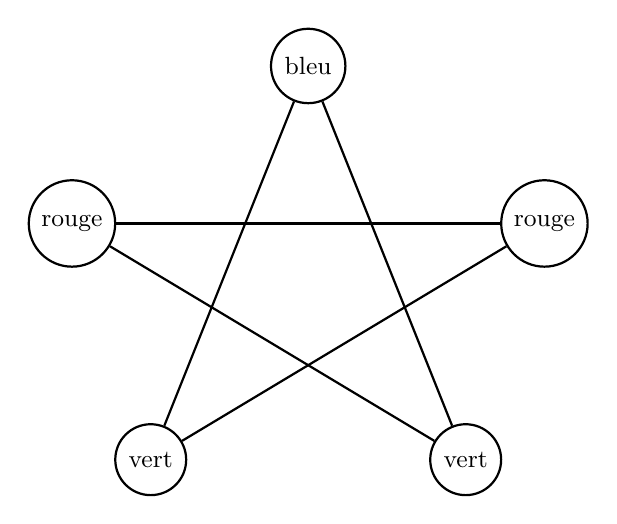
\begin{tikzpicture}
             \begin{scope}[every node/.style = {circle, thick, draw}]
                \node(1) at (0,0) {\small bleu};
                \node(2) at (3,-2) {\small rouge};              
                \node(3) at (2,-5) {\small vert};              
                \node(4) at (-2,-5) {\small vert};              
                \node(5) at (-3,-2) {\small rouge};               
            \end{scope}
           
            \begin{scope}[every edge/.style = {-, draw, thick}]
                \path(1) edge[] (4);
                \path(1) edge[] (3);
                \path(5) edge[] (3);
                \path(5) edge[] (2);
                \path(4) edge[] (2);
            \end{scope}
        \end{tikzpicture}
        \caption{Graphe 1}
    \end{subfigure}
    \hspace{2cm}
    \begin{subfigure}[b]{.3\linewidth}
        \centering
        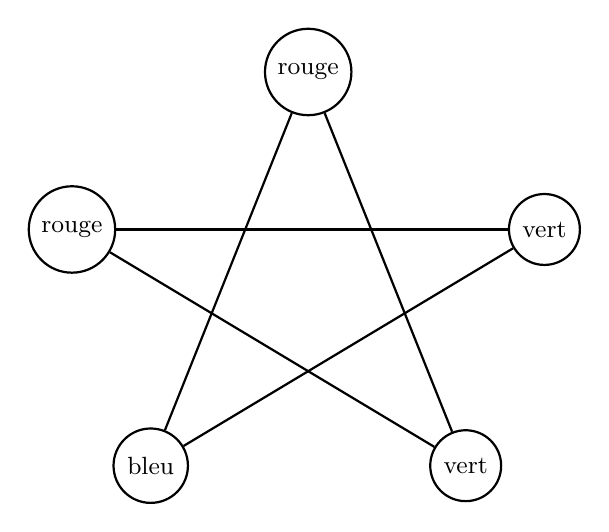
\begin{tikzpicture}
             \begin{scope}[every node/.style = {circle, thick, draw}]
                \node(1) at (0,0) {\small rouge};
                \node(2) at (3,-2) {\small vert};              
                \node(3) at (2,-5) {\small vert};              
                \node(4) at (-2,-5) {\small bleu};              
                \node(5) at (-3,-2) {\small rouge};                
            \end{scope}
            
            \begin{scope}[every edge/.style = {-, draw, thick}]
                \path(1) edge[] (4);
                \path(1) edge[] (3);
                \path(5) edge[] (3);
                \path(5) edge[] (2);
                \path(4) edge[] (2);
            \end{scope}
        \end{tikzpicture}
        \caption{Graphe 2}
    \end{subfigure}
    \caption{Deux graphes étiquettés}
    \label{fig:part1:graph}
    \hfill
\end{figure}

En appliquant la définition de graphe colorié, on remarque que pour le graphe 1, deux sommets étiquettés "rouge" sont voisins. Le graphe n'est donc pas colorié.\\
Pour ce qui est du graphe 2, en appliquant la définition, et en vérifiant pour tous les sommets, on voit qu'il est colorié car il n'existe pas deux sommets voisins de même couleur.

\subsection{}

\begin{figure}[H]
    \centering
    \begin{tikzpicture}
        \begin{scope}[every node/.style = {circle, thick, draw}, every edge/.style = {-, draw, thick}]
            \graph[math nodes, clockwise]
                { subgraph I_n [V={0,1,2,3,4}] --
                  subgraph C_n [V={5,6,7,8,9},radius=1.25cm];
                  {[cycle] 0,2,4,1,3} };
        \end{scope}
    \end{tikzpicture}
    \caption{Graphe de Petersen}
    \label{fig:part1:peterson}
\end{figure}

Rappelons que le nombre chromatique $\chi$ d'un graphe $G$ est le nombre minimal de couleurs nécessaires à colorier le graphe $G$. On notera par la suite $\chi(G)$ le nombre chromatique de $G$.\\
Rappelons aussi l'inégalité suivante (Théorème de Brooks) : 
\begin{equation}
    \omega(G) \leq \chi(G) \leq \Delta(G) + 1
\end{equation}
$\omega(G)$ est ici le nombre de sommets dans la clique maximale de $G$. Notons que déterminer la clique maximale d'un graphe est un problème \texttt{NP-hard}. Nous appelons clique un sous-graphe complet $K$ de $G$. Un graphe est dit complet si tout ses sommets sont adjacents deux à deux.\\
$\Delta(G)$ est ici le degré maximal du graphe, c'est-à-dire le nombre d'arêtes maximale que possède un sommet. Le $+1$ vient dans le cas où le graphe est cyclique impaire.\\
Pour le graphe de Peterson $P$, nous avons les résultats suivants : 
\begin{itemize}
    \item $\omega(P) = 2$ (on observe que $P$ ne contient pas de $K_3$ -- triangle)
    \item $\delta(P) = 3$
\end{itemize}
D'où d'après le Théorème de Brooks : 
\begin{itemize}
    \item $2 \leq \chi(P) \leq 4$ 
\end{itemize}
Toutefois, on observe que $P$ n'est pas $2$-colorable. En effet, supposons qu'il le soit. On observe que $P$ contient un sous-graphe cyclique impair $C$. 
On pose $C = \brac{S^1,A^1}$, tel que $S^1 = \{ 0,5,3,8,9 \}$ et $A^1 = \{ (0,3), (3,8), (8,9), (9,5), (5,0) \}$. Clairement, $C$ n'est pas $2$-colorable, mais il est en revanche 3-colorable.\\
Donc $P$ n'est pas $2$-colorable. Soit $R$ l'ensemble des sommets de couleur $r$, $B$ l'ensemble des sommets de couleur $b$ et $V$ l'ensemble des sommets de couleur $v$. On a alors (sans unicité du résultat) :
\begin{align*}
    V &= \{ 5,1,2,8 \}\\
    R &= \{ 7,3,4 \}\\
    B &= \{ 0,9,6 \}
\end{align*}
Ces trois ensembles forment bien un coloriage de $P$ : aucun sommet de $V$ n'est relié à un autre sommet de $V$ (de même pour $R$ et $B$). 
Donc $\chi(P) = 3$.


\subsection{}

\begin{algorithm}

\caption{Algorithme vérifiant si un étiquettage est un coloriage}
\label{alg:two}

\KwData{$G = \brac{S,A}$ un graphe et $L$ un étiquettage de $G$}
\KwResult{Si $L$ est un coloriage de $G$}
\textbf{Return:} \texttt{True} si $L$ est un coloriage, \texttt{False} sinon\\

bool res $\gets$ \texttt{True}\;

\If{$\lvert L \rvert < \lvert G \rvert$}{
    \Return{\texttt{False}}
}


\For{$v\in L$}{
    \For{$u\in L$}{
        \If{(couleur($x$) = couleur($y$)) et ($(x,y) \in A$)}{
            res $\gets$ \texttt{False}\;
        }
    }
}
\Return{res}
\end{algorithm}

\lstinputlisting{parts/annexe/code/coloriage_3.cpp}


\subsection{}

Rappelons que le nombre maximal de couleur pour colorier un graphe à $n$ sommets est $n$ couleurs.
L'idée ici est d'énumerer toutes les colorations possibles, jusqu'à trouver une coloration valide. Soit $G = \brac{S,A}$ un graphe, tel que $\lvert S \rvert = n$. Montrons que l'algorithme $\mathcal{A}$ qui trouve le nombre chromatique de ce graphe est exponentiel en temps dans le pire des cas.
\\
On teste si $G$ est $k$-colorable, pour $k$ allant de $2$ à $n-1$. $G$ ayant $n$ sommets, pour chaque valeur de $k$ il y a $k^n$ coloriages possibles.
Le nombre de coloriage possible est alors donné par la formule suivante : 
\begin{align}
    \sum^{n-1}_{k = 2} k^n &= 2^n + ... + (n-1)^n\\
    &< \sum_{k=2}^{n-1} (n-1)^n \\
    &< (n-1)\times (n-1)^n\\
    &< (n-1) e^{n \log (n-1)}
\end{align}
De plus, chaque etiquetage nécessite $\comp{n^2}$ pour être testé (question 1.3). On a donc la borne de complexité suivante : 
$\comp{n^2(n-1) e^{n \log(n-1}}$. La complexité est bien exponentielle.